\chapter{\IfLanguageName{dutch}{Stand van zaken}{State of the art}}%
\label{ch:stand-van-zaken}

% Tip: Begin elk hoofdstuk met een paragraaf inleiding die beschrijft hoe
% dit hoofdstuk past binnen het geheel van de bachelorproef. Geef in het
% bijzonder aan wat de link is met het vorige en volgende hoofdstuk.

% Pas na deze inleidende paragraaf komt de eerste sectiehoofding.

\section{Natural Language Processing: Een Overzicht en Toepassingen}

Natural Language Processing (NLP) speelt een essentiële rol bij de interactie tussen computers en menselijke talen. Dit hoofdstuk vormt een basis voor het begrijpen van AI-modellen, cruciaal voor het ontwikkelen van een privacybewust spelling- en grammaticacontroletoetsenbord voor Android. Het vormt de grondslag voor latere bespreking van specifieke AI-modellen en hun toepassingen.


\subsection{Definitie en Belang van NLP}

Natural Language Processing is een cruciale subdiscipline binnen de artificiële intelligentie die zich richt op de interactie tussen computers en menselijke (natuurlijke) talen. Het stelt machines in staat om menselijke taal te begrijpen en interpreteren, wat essentieel is voor het efficiënt verwerken van grote hoeveelheden tekstuele en spraakgegevens. De ontwikkeling van NLP heeft de manier waarop machines menselijke taal analyseren fundamenteel veranderd, w\-aar\-door ze niet alleen tekst kunnen begrijpen maar, ook reageren in een manier die voorheen voorbehouden was aan menselijke interactie \autocite{Sanadi2022}.

\subsection{Hoe NLP werkt}

Natural Language Processing combineert linguïstiek, computerwetenschap en artificiële intelligentie om machines in staat te stellen menselijke taal te begrijpen, interpreteren en genereren. De werking van NLP kan worden onderverdeeld in verschillende belangrijke stappen, die hieronder worden beschreven.

\begin{itemize}
    \item \textbf{Taalkundige Voorverwerking}: Dit is de eerste stap in NLP, waarbij ruwe tekst wordt omgezet in een meer gestructureerde vorm die geschikt is voor verdere analyse. Het omvat verschillende processen zoals tokenisatie, waarbij tekst wordt opgedeeld in kleinere eenheden zoals woorden of zinnen, en normalisatie, waarbij tekst wordt gestandaardiseerd door het verwijderen van leestekens, het omzetten van hoofdletters naar kleine letters, en het corrigeren van spelfouten.
    
    \item \textbf{Syntactische Analyse}: Deze stap omvat het analyseren van de grammaticale structuur van zinnen. Dit wordt vaak gedaan door middel van parsing, waarbij een boomstructuur wordt gecreëerd die de relaties tussen woorden binnen een zin weergeeft. Door syntactische analyse kan een systeem de structuur van een zin begrijpen, wat helpt bij het ontleden van de betekenis ervan.
    
    \item \textbf{Semantische Analyse}: Bij semantische analyse wordt de betekenis van woorden en zinnen afgeleid. Dit gaat verder dan syntactische analyse door de daadwerkelijke betekenis van de tekst te interpreteren. Het omvat taken zoals woordenschat disambiguatie, waarbij de juiste betekenis van een woord wordt bepaald op basis van de context, en het genereren van synoniemen en parafraseringen.
    
    \item \textbf{Pragmatische Analyse}: Dit onderdeel van NLP houdt rekening met de context waarin taal wordt gebruikt, inclusief de intentie van de spreker en de omgevingsfactoren die van invloed kunnen zijn op de interpretatie. Pragmatische analyse helpt bij het begrijpen van de impliciete betekenissen en nuances in de communicatie.
    
    \item \textbf{Machine Learning en Deep Learning}: Moderne NLP-modellen maken vaak gebruik van machine learning en deep learning technieken om tekst te verwerken en te begrijpen. Modellen zoals neurale netwerken en transformerarchitecturen (bijvoorbeeld BERT en GPT) worden getraind op grote hoeveelheden tekstgegevens om patronen en structuren in taal te leren herkennen. Deze modellen kunnen vervolgens worden toegepast op een breed scala aan NLP-taken, zoals vertaling, sentimentanalyse, en tekstgeneratie.
    
    \item \textbf{Evaluatie en Feedback}: Na de initiële verwerking en analyse, worden de resultaten geëvalueerd en indien nodig bijgesteld. Dit omvat het meten van de prestaties van het model en het verbeteren van de nauwkeurigheid door middel van iteratieve training en fine-tuning. Feedback van gebruikersinteracties kan ook worden gebruikt om de prestaties van NLP-systemen verder te verbeteren.
\end{itemize}

Door deze stappen te combineren, kan NLP effectief menselijke taal begrijpen en erop reageren, wat essentieel is voor toepassingen zoals een privacybewust spelling- en grammaticacontroletoetsenbord. Lokale verwerking op apparaten biedt hierbij extra voordelen door de privacy van gebruikers te beschermen en het risico op datalekken te minimaliseren \autocite{Hirschberg2015}.

\subsection{Toepassingen van NLP}

De toepassingen van NLP zijn divers en invloedrijk in verschillende domeinen, van machine vertaling en sentiment analyse tot stemgestuurde assistenten. Deze technologieën worden steeds vaker geïmplementeerd in apparaten en diensten die we dagelijks gebruiken, wat aantoont hoe diepgaand NLP de interactie tussen mens en machine heeft getransformeerd. Door de integratie van NLP in deze applicaties kunnen apparaten complexe menselijke commando's begrijpen en hierop reageren, wat de bruikbaarheid en toegankelijkheid van technologie verbetert \hfill \break \autocite{Feng2020}.

\subsection{Privacyvoordelen van Lokale NLP}

Een belangrijke ontwikkeling binnen NLP is de implementatie van deze technologieën direct op lokale apparaten, zoals Android smartphones. Door NLP lokaal uit te voeren, kunnen gebruikers profiteren van de voordelen die bij taalverwerking komen, zonder hun gegevens naar externe servers te sturen. Dit voorziet ons van aanzienlijke privacyvoordelen, aangezien gevoelige informatie op het apparaat zelf wordt verwerkt en beheerd, waardoor het risico op datalekken en externe toegang tot persoonlijke gegevens wordt verminderd. \textcite{Guo2022} benadrukken hoe NLP-inferentie op het apparaat zelf cruciaal is voor het behoud van de privacy bij gebruikersgegevens door het vermijden van netwerkverkeer. Deze benadering is vooral belangrijk in toepassingen waarbij gevoelige gegevens worden verwerkt, zoals in medische, financiële of persoonlijke assistent-applicaties \autocite{Locke2021Natural}.
\\ \\
De integratie van NLP in zowel dagelijkse als gespecialiseerde technologieën heeft aanzienlijke voordelen voor het begrijpen en verwerken van menselijke taal. Door deze systemen lokaal te implementeren, kunnen ontwikkelaars en eindgebruikers genieten van zowel functionele als privacy-voordelen, wat essentieel is in onze s\-t\-ee\-ds meer verbonden en gegevensgevoelige wereld.

\section{AI-Modellen voor Mobiele Apparaten: Een Focus op BERT, DistilBERT en TinyBERT}

Dit hoofdstuk bouwt voort op de basis van NLP en bespreekt AI-modellen zoals BERT, DistilBERT en TinyBERT, die essentieel zijn voor NLP-toepassingen op mobiele apparaten. Deze kennis helpt bij het selecteren en optimaliseren van de juiste modellen voor de toetsenbordapplicatie.

\subsection{Overzicht van Modellen}

Recente ontwikkelingen in AI-modellen hebben geleid tot aanzienlijke vooruitgang in natuurlijke taalverwerking. Modellen zoals BERT (Bidirectional Encoder Representations from Transformers) en zijn afgeleiden, DistilBERT en TinyBERT, spelen een cruciale rol. BERT-modellen zijn met name effectief in het begrijpen van de context gericht op woorden binnen een zin, wat hen zeer geschikt maakt voor complexe NLP-taken. Echter, vanwege hun grootte en complexiteit, zijn deze modellen vaak niet direct geschikt voor gebruik op mobiele apparaten met beperkte bronnen. Om dit probleem aan te pakken, zijn DistilBERT en TinyBERT ontwikkeld als kleinere, efficiëntere versies die beter geschikt zijn voor mobiele toepassingen. TinyBERT, bijvoorbeeld, is speciaal ontworpen voor kennisdestillatie van Transformer-gebaseerde modellen, wat resulteert in een model dat aanzienlijk kleiner en sneller is dan zijn voorganger, zonder aanzienlijke compromissen in de prestaties \autocite{Jiao2019TinyBERT}.

\subsection{Criteria voor Modelkeuze}

Bij het kiezen van een taalmodel voor mobiele apparaten zijn er enkele belangrijke criteria te overwegen, waaronder modelgrootte, nauwkeurigheid en de benodigde rekenkracht. Kleinere modellen zoals TinyBERT en DistilBERT zijn vaak de voorkeursopties omdat ze minder opslagruimte en verwerkingscapaciteit vereisen. Deze modellen behouden een aanzienlijke mate van nauwkeurigheid, terwijl ze aanzienlijk sneller en lichter zijn, wat essentieel is voor toepassingen op mobiele apparaten \autocite{Sun2020MobileBERT}.

\subsection{Vergelijking van Modellen}

TinyBERT en DistilBERT bieden beide aanzienlijke voordelen ten opzichte van het oorspronkelijke BERT-model wat betreft inzetbaarheid op mobiele apparaten. TinyBERT, bijvoorbeeld, biedt vergelijkbare prestaties als BERT-Base maar met slechts 28\% van de parameters en 31\% van de inferentietijd. DistilBERT daarentegen behoudt ongeveer 97\% van de taalbegripscapaciteit van BERT, terwijl het 40\% kleiner is en 60\% sneller dan het originele BERT-model. Deze modellen illustreren hoe kennisdestillatie kan worden gebruikt om krachtige, doch lichte modellen te creëren die geschikt zijn voor gebruik in resource-beperkte omgevingen zoals mobiele apparaten \autocite{Sanh2019DistilBERT}.


\section{BERT, RobBERT, en RobBERTje: Prestaties en Optimalisaties van Nederlandse Taalmodellen}

Voortbouwend op de bespreking van AI-modellen, richt dit hoofdstuk zich op Nederlandse varianten zoals RobBERT en RobBERTje. We onderzoeken hun prestaties en optimalisaties, wat cruciaal is voor de implementatie van effectieve taalmodellen in de toetsenbord applicatie.

\subsection{Inleiding tot BERT}

BERT (Bidirectional Encoder Representations from Transformers) is een trans\-for\-mer-gebaseerd model dat heeft gezorgd voor aanzienlijke verbeteringen in verschillende natuurlijke taaltaken door zijn vermogen om diepe bidirectionele representaties te pre-trainen. Dit model kan fijn afgesteld worden met slechts één extra outputlaag om toonaangevende resultaten te leveren voor een breed scala aan taken, zoals vraag beantwoording en taal inferentie, zonder substantiële aanpassingen in de taakspecifieke architectuur \autocite{Devlin2019}.

\subsection{Hoe BERT werkt}

BERT maakt gebruik van de Transformer, een aandachtsmechanisme dat helpt bij het begrijpen van de relaties tussen woorden in een tekst. De Transformer bestaat uit een encoder die de tekst leest en een decoder die voorspellingen doet.

In tegenstelling tot modellen die de tekst van links naar rechts of van rechts naar links lezen, leest de Transformer-encoder de complete reeks woorden tegelijkertijd. Dit maakt het mogelijk om de context van een woord te begrijpen op basis van de woorden eromheen.

\begin{figure}[ht]
    \centering
    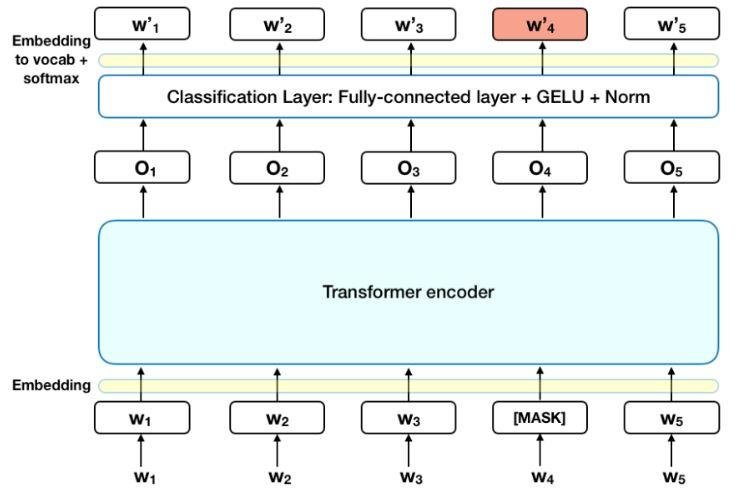
\includegraphics[width=0.8\textwidth]{bert_explained.jpg}
    \caption{Een overzicht van de Transformer-encoder door \autocite{Devlin2019}}
    \label{fig:bert_explained}
\end{figure}

Figuur \ref{fig:bert_explained} toont hoe de Transformer-encoder werkt. De invoer is een reeks woorden die worden omgezet in vectoren en vervolgens verwerkt worden in een neuraal netwerk. De uitvoer is een reeks vectoren, waarbij elke vector overeenkomt met een invoerwoord.

Bij het trainen van taalmodellen is het moeilijk om een goed voorspellingsdoel te bepalen. Veel modellen voorspellen het volgende woord in een zin, wat de context beperkt. BERT gebruikt twee trainingsstrategieën om dit probleem op te lossen:

\textbf{Masked LM (MLM)}: Voordat de woordreeksen in BERT worden ingevoerd, wordt 15\% van de woorden vervangen door een [MASK]-token. Het model probeert dan de oorspronkelijke woorden te voorspellen op basis van de context van de andere woorden in de reeks. Dit vereist:

\begin{itemize}
    \item Een classificatielaag bovenop de encoderuitvoer.
    \item Het vermenigvuldigen van de uitvoervectoren met de embedding-matrix om ze om te zetten naar vocabulaire-dimensies.
    \item Het berekenen van de waarschijnlijkheid van elk woord met softmax.
\end{itemize}

De verliesfunctie van BERT houdt alleen rekening met de voorspelling van de gemaskeerde woorden, wat leidt tot een langzamere convergentie maar beter contextbegrip.

\textbf{Next Sentence Prediction (NSP)}: BERT krijgt tijdens de training paren van zinnen en leert te voorspellen of de tweede zin volgt op de eerste. In 50\% van de gevallen volgt de tweede zin, en in de andere 50\% niet. Het model leert het verschil te herkennen door de invoer als volgt te verwerken:

\begin{itemize}
    \item Een [CLS]-token aan het begin en een [SEP]-token aan het einde van elke zin.
    \item Een zinsembedding die aangeeft of het de eerste of tweede zin is.
    \item Een positionele embedding die de positie in de reeks aangeeft.
\end{itemize}

Om te voorspellen of de tweede zin volgt op de eerste, worden de volgende stappen uitgevoerd:

\begin{itemize}
    \item De hele invoersequentie gaat door de Transformer.
    \item De uitvoer van het [CLS]-token wordt omgezet in een vector.
    \item De waarschijnlijkheid van IsNextSequence wordt berekend met softmax.
\end{itemize}

BERT traint Masked LM en Next Sentence Prediction samen om de gecombineerde verliesfunctie te minimaliseren \autocite{Devlin2019}.


\subsection{RobBERT en RobBERTje}

RobBERT en RobBERTje zijn Nederlandse varianten van het BERT-model, ontwikkeld om beter te presteren op taaltaken specifiek voor het Nederlands. RobBERT gebruikt een modelarchitectuur vergelijkbaar met die van BERT maar is getraind op een rijke dataset van Nederlandse teksten, wat resulteert in verbeterde prestaties op downstream NLP-taken zoals part-of-speech tagging en naamherkenning. RobBERTje is een verder gedistilleerde versie, gecreëerd met zicht op een efficiëntie in grote en snelheid voor mobiele toepassingen \autocite{Vries2019}.

\subsection{Vergelijking van Distillatiearchitecturen}

Distillatiearchitecturen zoals TinyBERT, DistilBERT en RobBERTje hebben elk unie\-ke benaderingen en optimalisaties die hen onderscheiden, vooral in hoe ze presteren en hoe ze worden getraind.

\textbf{TinyBERT} maakt gebruik van een tweefasig leerproces dat zowel tijdens de pre-training als taakspecifieke afstemming plaatsvindt. Deze methode zorgt ervoor dat TinyBERT zowel algemene als taakspecifieke kennis efficiënt kan overnemen van zijn 'leraar'-model. TinyBERT slaagt erin om met slechts 28\% van de parameters en 31\% van de inferentietijd vergeleken met zijn leraar, BERT-Base, toch meer dan 96.8\% van de prestaties te behouden op de GLUE benchmark. Deze indrukwekkende reductie in grootte en snelheid maakt TinyBERT bijzonder geschikt voor mobiele en ingebedde toepassingen \autocite{Jiao2019TinyBERT}.

\textbf{DistilBERT}, aan de andere kant, is ontworpen om de grootte van het BERT-model met 40\% te verminderen, terwijl nog steeds 97\% van zijn taalbegripscapaciteiten behouden blijft. Dit wordt bereikt door kennisdestillatie toe te passen tijdens de pre-trainingsfase. DistilBERT gebruikt een 'triple loss' die taalmodellering, distillatie en cosinusafstandsverlies combineert, wat bijdraagt aan een efficiënte overdracht van kennis en een snellere inferentie, waardoor het een kosteneffectieve keuze is voor op apparaat gebaseerde berekeningen \autocite{Sanh2019DistilBERT}.

\textbf{RobBERTje} richt zich op het optimaliseren van de Nederlandse taalmodellen door verschillende distillatiecorpora te onderzoeken. Dit onderzoek heeft aangetoond dat het mengen van opeenvolgende zinnen in een corpus kan leiden tot modellen die sneller trainen en beter presteren op taken met lange sequenties. Dit suggereert dat de structuur van het trainingscorpus aanzienlijk kan bijdragen aan de effectiviteit van gedistilleerde modellen. Interessant is dat RobBERTje ook minder genderstereotype bias vertoont dan zijn leraarsmodel, wat wijst op een bijkomend voordeel van het distillatieproces \autocite{Delobelle2021}.

Deze diverse benaderingen van modeldistillatie illustreren de veelzijdigheid en aanpasbaarheid van distillatiearchitecturen in het verkleinen en versnellen van trans\-for\-mer-gebaseerde modellen, terwijl nog steeds een hoge mate van nauwkeurigheid behouden blijft. Elk van deze modellen heeft unieke voordelen, afhankelijk van de specifieke eisen en beperkingen van de toepassing, zoals geheugenbeperkingen, rekenkracht, en de specifieke kenmerken van de taak of het taaldomein.


\subsection{Bias en Efficiëntie}

Ondanks de efficiëntievoordelen van gedistilleerde modellen zoals RobBERTje, is het belangrijk om aandacht te besteden aan de bias die deze modellen kunnen bevatten. Het minimaliseren van bias terwijl de efficiëntie wordt gemaximaliseerd, blijft een belangrijk aandachtspunt voor de ontwikkeling van toekomstige NLP-modellen. Efficiëntie in training en inferentie is cruciaal voor de bruikbaarheid van deze modellen in real-world toepassingen, vooral op mobiele apparaten waar rekenkracht en geheugen beperkt zijn.


\section{Privacy en Gegevensbescherming}

Na de bespreking van taalmodellen en hun optimalisaties, verschuift dit hoofdstuk de focus naar privacy en gegevensbescherming. We bespreken waarom lokale verwerking belangrijk is voor privacy en hoe gevoelige gegevens veilig kunnen worden verwerkt, wat essentieel is voor een privacybewust toetsenbord.

\subsection{Belang van Privacy}

Lokale verwerking van gegevens wordt steeds belangrijker voor privacy en gegevensbescherming, vooral in het tijdperk van Internet der Dingen (IoT) en edge computing. Door gegevens lokaal te verwerken, wordt de noodzaak voor gegevensoverdracht over het netwerk verminderd, wat niet alleen de efficiëntie verbetert maar ook het risico op gegevenslekken vermindert. Dit is essentieel in situaties waar de privacy van gebruikers cruciaal is, zoals in gezondheidszorg en financiële diensten \autocite{Bi2020}.

\subsection{Gevoelige Data Verwerking}

Het beheren van gevoelige gegevens vereist een zorgvuldige aanpak om privacy van de gebruiker te waarborgen. Best practices omvatten het gebruik van data-encryptie en veilige communicatieprotocollen om te verzekeren dat gegevens tijdens de overdracht en opslag beschermd zijn. Technieken zoals de Advanced Encryption Standard (AES) en Secure Sockets Layer (SSL) zijn cruciaal voor het veilig overbrengen en opslaan van gegevens. Daarnaast is de implementatie van lokale differentiële privacytechnieken een effectieve manier om te zorgen voor anonimiteit van gegevens, terwijl de bruikbaarheid van ervan behouden blijft \autocite{Shah2014}.

\subsection{Privacy-overwegingen}

Bij het ontwerpen van systemen die gevoelige gegevens verwerken, moeten ontwikkelaars diverse privacy-overwegingen in acht nemen. Dit omvat het minimaliseren van gegevensverzameling, het verzekeren van transparantie over hoe gegevens worden gebruikt, en het implementeren van robuuste toegangscontrolesystemen. Het is ook belangrijk om privacy by design-principes te adopteren, wat betekent dat privacybescherming vanaf het begin geïntegreerd wordt bij het systeemontwerp. Methoden zoals het minimaliseren van de verzamelde gegevens en het verzekeren van een sterke gebruikerstoestemming voor het gebruik van hun gegevens zijn essentieel voor het handhaven van vertrouwen en integriteit in data gedreven systemen \autocite{Edwards2019}.


\section{Huidige Oplossingen en Beperkingen}

Gebaseerd op de eerdere bespreking van privacy en modeloptimalisatie, onderzoekt dit hoofdstuk bestaande methoden voor AI-integratie op mobiele apparaten. We analyseren de voor- en nadelen van huidige oplossingen om inzicht te krijgen in de beperkingen en kansen voor verbetering.

\subsection{Bestaande Methoden}

\textbf{Spraakherkenning op Mobiele Apparaten:}
Spraakherkenningstechnologie, aangedreven door AI, is aanzienlijk verbeterd en wordt gebruikt in diverse toepassingen zoals virtuele assistenten, spraak gestuurde apparaten en dicteer software. De\-ze technologie maakt gebruik van machine learning-algoritmen die getraind zijn op grote hoeveelheden spraakgegevens om menselijke spraak te herkennen en interpreteren met nauwkeurigheidsniveaus die vergelijkbaar zijn met die van mensen. Automatische spraakherkennings(ASR)-systemen bestaan uit drie hoofdcomponenten: het akoestische model, het taalmodel en de decoder. Deze componenten werken samen om gesproken input te verwerken in geschreven tekst, ondanks uitdagingen zoals spraakvariatie en achtergrondlawaai \autocite{Wang2023}.
\\ \\
\textbf{Beeldverwerking op Mobiele Apparaten:}
AI wordt ook uitgebreid toegepast in de beeldverwerking op mobiele apparaten, voornamelijk voor functies zoals gezichtsherkenning en objectdetectie. Deze systemen gebruiken diepe leermodellen die zijn geoptimaliseerd voor mobiele apparaten om complexe beeldverwerkingstaken uit te voeren. Door gebruik te maken van convolutionele neurale netwerken (CNN's) kunnen deze modellen patronen in visuele gegevens herkennen en interpreteren, wat van cruciaal belang is voor toepassingen zoals fotografie-apps, gezondheidsmonitoring en interactieve gaming \autocite{Luo2018}. Bovendien versterken geavanceerde AI-strategieën de mogelijkheden van mobiele applicaties door contextbewustzijn en adaptief leren te bieden, wat essentieel is voor gepersonaliseerde gebruikerservaringen \autocite{Sarker2021}.

\subsection{Voor- en Nadelen}

\textbf{Voordelen} van deze AI-toepassingen omvatten de mogelijkheid om complexe en natuurlijke interacties met apparaten te faciliteren, wat leidt tot een verbeterde gebruikerservaring. Door lokale verwerking kunnen deze toepassingen ook werken met minimale vertraging en verhoogde privacy voor de gebruiker.
\\ \\
\textbf{Nadelen} zijn onder meer de beperkingen in verwerkingskracht en batterijduur van mobiele apparaten, wat de complexiteit en efficiëntie van de uitvoerbare AI-modellen beperkt. Bovendien kunnen deze systemen te maken krijgen met uitdagingen zoals onnauwkeurigheden in moeilijke omgevingscondities en de noodzaak van continue updates om de modellen te verbeteren en adapteren aan nieuwe data \autocite{Castanyer2021}.


\section{Model Conversie en Optimalisatie}

In navolging van de analyse op huidige oplossingen, bespreekt dit hoofdstuk de stappen voor modelconversie en optimalisatietechnieken. Deze technieken zijn cruciaal voor de efficiënte integratie van AI-modellen op mobiele apparaten, zoals besproken in de vorige hoofdstukken.


\subsection{Model Conversie}

Het converteren van AI-modellen naar formaten die compatibel zijn met mobiele apparaten is een cruciale stap om de implementatie van machine learning in mobiele applicaties te faciliteren. Veelgebruikte formaten voor compatibiliteit omvatten TensorFlow Lite en ONNX (Open Neural Network Exchange). TensorFlow Lite is een lichtgewicht oplossing die speciaal is ontworpen voor mobiele en ingebedde apparaten, en voorziet tools die modellen optimaliseren voor on-device uitvoering. ONNX daarentegen is een open formaat dat ontworpen is om modelportabiliteit en interoperabiliteit te ondersteunen, zodat ontwikkelaars modellen kunnen gebruiken over verschillende frameworks en tools heen zonder dat modelconversie nodig is. Dit proces omvat gewoonlijk het vereenvoudigen, verminderen van de grootte, en verzekeren dat het model efficiënt werkt binnen de beperkingen van een mobiel apparaat \autocite{Dalwadi2021}.

\subsection{Optimalisatietechnieken}

Naast conversie zijn geavanceerde optimalisatietechnieken essentieel om de prestaties van AI-modellen op mobiele apparaten te verbeteren. Deze omvatten:

\begin{enumerate}
    \item \textbf{Kwantisatie}: Dit proces converteert een model van drijvende-komma\-getal\-in\-de\-ling naar een gehele getallen indeling, wat de modelgrootte vermindert en de inferentie snelheid verhoogt zonder significante verlies van nauwkeurigheid. Verschillende vormen van kwantisatie, zoals uniforme en niet-uniforme, kunnen worden toegepast, afhankelijk van de specifieke vereisten van de toepassing \autocite{Wang2022}.
    
    \item \textbf{Snoeien}: Door onnodige, redundante of minder belangrijke gewichten uit het neurale netwerk te verwijderen, vermindert snoeien de complexiteit en grootte van het model, wat resulteert in snellere verwerkingstijden. Deze techniek kan zowel gestructureerd als ongestructureerd worden toegepast om verschillende niveaus van compressie te bereiken, afhankelijk van de doelstellingen met betrekking tot modelprestatie en -compressie.
    
    \item \textbf{Clustering}: Deze techniek groepeert de gewichten van het neurale netwerk in een beperkt aantal clusters om de algehele grootte van het model te verminderen en de inferentie snelheid te verhogen. Clustering kan worden gecombineerd met kwantisatie om verdere compressie en prestatieverbeteringen te bereiken \autocite{Ye2018}.
\end{enumerate}

Deze technieken dragen bij aan de efficiëntie van AI-modellen door het verminderen van hun rekenlast en geheugenvereisten, waardoor ze beter geschikt zijn voor gebruik op mobiele apparaten met beperkte resources.


\section{Integratie van het Model in een Android Applicatie}

Na de bespreking van modelconversie en optimalisatie, richt dit hoofdstuk zich op de praktische aspecten met betrekking tot het integreren van AI-modellen in Android-applicaties. We behandelen de frameworks en tools die nodig zijn voor deze integratie, evenals technieken voor preprocessing, postprocessing en prestatieoptimalisatie.

\subsection{Mobiel-vriendelijke Deep Learning Frameworks en Tools}

Voor de integratie van AI-modellen op Android-apparaten zijn TensorFlow Lite en ONNX Runtime de meest prominente frameworks, ontworpen om modelcompatibiliteit en efficiënte uitvoering op mobiele en embedded apparaten te ondersteunen. TensorFlow Lite optimaliseert modellen specifiek voor snelle prestaties met beperkte middelen, terwijl ONNX Runtime een efficiënte modelinfrastructuur bie\-dt die de interoperabiliteit tussen verschillende frameworks zoals PyTorch en TensorFlow bevordert. Deze faciliteren niet alleen hardwareversnelling die essentieel is voor diepe neurale netwerken, maar bieden ook uitgebreide API's die eenvoudig te integreren zijn in de Android ontwikkelomgeving voor standaard modelinvoer, -inferentie en -uitvoer. Voor custom modellen, vooral die complexe tekstuele inferentie vereisen, zijn de beschikbare middelen echter beperkt en is er vaak aanzienlijke aanpassing nodig. Dit kan een leercurve voor ontwikkelaars verhogen vanwege de beperkte documentatie die specifieke implementatiedetails behandelt \autocite{Openja2022}.

\subsection{Preprocessing en Postprocessing}

Data preprocessing omvat het formatteren en normaliseren van invoergegevens zodat deze compatibel zijn met het AI-model. Voor beeldverwerking kan dit inhouden dat afbeeldingen worden geschaald of genormaliseerd naar een specifiek kleurbereik. Postprocessing aan de andere kant, richt zich op het interpreteren van de modeloutput, zoals het omzetten van ruwe scores naar bruikbare inzichten of beslissingen.

\subsection{Prestaties en Batterijoptimalisatie}

Het optimaliseren van prestaties en batterijduur is cruciaal voor mobiele applicaties. Technieken zoals kwantisatie, het gebruik van efficiënt geheugenbeheer en het minimaliseren van de achtergrondactiviteiten kunnen helpen om de energie-efficiëntie te verbeteren en de responsiviteit ervan te verhogen. Caching van frequente query's en het slim plannen van achtergrondtaken kunnen ook bijdragen aan een langere batterijduur en een soepelere gebruikerservaring.


\section{Soorten Android-diensten}

Dit hoofdstuk bouwt voort op de praktische integratie van AI-modellen en bespr\-eekt verschillende soorten Android-diensten zoals IME en System-level Services. We onderzoeken hun voordelen, nadelen en implementatiestappen, wat helpt bij het begrijpen van de infrastructuur waarin AI-modellen kunnen worden geïmplementeerd.


\subsection{Android Input Method Editor (IME)}

De Android Input Method Editor (IME) is een programma dat gebruikers in staat stelt tekens en symbolen in te voeren op mobiele apparaten. IME's zijn vooral belangrijk voor talen met uitgebreide karakters, zoals Chinees, Japans en Koreaans.

\subsubsection{Voordelen en Nadelen}

\textbf{Voordelen}:
\begin{itemize}
    \item \textbf{Gebruiksvriendelijkheid}: IME's verbeteren de tekstinvoersnelheid en -nauw\-keu\-rig\-heid door voorspellende tekst en automatische correctie te bieden, wat de algehele gebruikerservaring verbetert.
    \item \textbf{Flexibiliteit}: Ze voorzien ondersteuning voor meerdere talen en aangepaste toetsenbord lay-outs, waardoor ze breed inzetbaar zijn voor diverse gebruikersbehoeften.
    \item \textbf{Personalisatie}: IME's kunnen worden aangepast op basis van gebruikersgedrag en voorkeuren, wat resulteert in een meer gepersonaliseerde gebruikerservaring \autocite{Jo2015}.
\end{itemize}

\textbf{Nadelen}:
\begin{itemize}
    \item \textbf{Privacyrisico's}: Omdat IME's toegang hebben tot alle getypte gegevens, kunnen ze gevoelige informatie blootstellen aan privacyrisico's, vooral als de IME op een cloud gehost wordt \autocite{Kawamoto2014}.
    \item \textbf{Prestatie}: Sommige IME's kunnen de prestaties van apparaten beïnvloeden door verhoogd geheugen- en CPU-gebruik.
    \item \textbf{Beveiligingsrisico's}: IME's zijn kwetsbaar voor beveiligingsproblemen zoals keylogging en gegevensinbreuken, vooral wanneer derde partijen betrokken zijn \autocite{Diao2015}.
\end{itemize}

\subsubsection{Implementatiestappen}

\begin{enumerate}
    \item \textbf{Opzetten van het IME Framework}: Begin met het instellen van de basisstructuur door benodigde Android API's te integreren.
    \item \textbf{Ontwikkeling van het Toetsenbordinterface}: Ontwerp en implementeer het toetsenbordinterface, inclusief de lay-out en interactie-elementen.
    \item \textbf{Integratie van Taalmodellen}: Voeg voorspellende tekst- en autocorrectiefuncties toe door modellen te integreren
    \item \textbf{Testen en Optimaliseren}: Voer uitgebreide tests uit om de prestaties, nauwkeurigheid en beveiliging van het IME te waarborgen.
    \item \textbf{Publicatie en Onderhoud}: Publiceer de IME op Google Play Store en zorg voor regelmatige updates en onderhoud om bugs en beveiligingsproblemen aan te pakken.
\end{enumerate}

\subsection{Android System-level Service}

Android System-level Services zijn processen die op systeemniveau draaien en die door meerdere applicaties kunnen worden gebruikt. Ze bieden belangrijke functies zoals locatiebepaling, netwerkbeheer en gegevenssynchronisatie.

\subsubsection{Voordelen en Nadelen}

\textbf{Voordelen}:
\begin{itemize}
    \item \textbf{Hoge Efficiëntie}: System-level services zijn geoptimaliseerd voor prestaties en kunnen efficiënt functioneren zonder significante impact op de systeembronnen.
    \item \textbf{Gedeelde Functionaliteit}: Deze services kunnen door meerdere applicaties worden gebruikt, wat redundantie vermindert en de consistentie verbetert.
    \item \textbf{Betere Integratie}: System-level services kunnen naadloos integreren met andere systeemcomponenten, wat resulteert in een meer coherente gebruikerservaring.
\end{itemize}

\textbf{Nadelen}:
\begin{itemize}
    \item \textbf{Complexiteit van Implementatie}: Het opzetten van systeemdiensten vereist diepgaande kennis van het Android-platform en kan complex zijn.
    \item \textbf{Beperkte Toegang}: Omdat systeemdiensten op een hoger beveiligingsniveau draaien, hebben ze beperkte toegang tot bepaalde gebruikersgegevens en -functies.
    \item \textbf{Moeilijkheid bij Debuggen}: Problemen met systeemdiensten kunnen soms moeilijker te debuggen zijn vanwege hun integratie op laag niveau met het besturingssysteem.
\end{itemize}

\subsubsection{Implementatiestappen}

\begin{enumerate}
    \item \textbf{Definiëren van de Service}: Stel de specificaties en functionaliteiten van de systeemdienst vast.
    \item \textbf{Ontwikkeling van de Service}: Gebruik de Android API's om de basisstructuur en functionaliteit van de service te implementeren.
    \item \textbf{Integratie met Systeemcomponenten}: Zorg voor integratie van de service met andere relevante systeemcomponenten.
    \item \textbf{Testen en Optimaliseren}: Voer grondige tests uit om ervoor te zorgen dat de service stabiel, efficiënt en veilig is.
    \item \textbf{Implementatie en Onderhoud}: Implementeer de service op apparaten en zorg voor regelmatig onderhoud en updates om optimale prestaties te garanderen.
\end{enumerate}


\section{Case Studies en Voorbeelden}

Het laatste hoofdstuk presenteert case studies en voorbeelden van mobiele applicaties die AI-modellen lokaal draaien. We analyseren succesverhalen en mislukkingen, waaruit belangrijke lessen voor toekomstige implementaties komen. Dit helpt bij het contextualiseren van de besproken technologieën en brengt praktische inzichten voor de toepassing van deze bachelorproef.


\subsection{Relevante Voorbeelden}

Er zijn verschillende voorbeelden van mobiele applicaties die AI-modellen lokaal draaien, met zowel succesverhalen als mislukkingen.

\textbf{Succesverhalen}:
\begin{itemize}
    \item \textbf{Google Translate}: Google Translate maakt gebruik van een offline modus waarbij neurale machinevertalingsmodellen lokaal op het apparaat worden uitgevoerd. Dit verbetert de vertalingskwaliteit aanzienlijk en geeft gebruikers snelle en betrouwbare vertalingen zonder een internetverbinding. Dit succes is te danken aan de optimalisatie van AI-modellen voor mobiele apparaten, waardoor ze efficiënt werken binnen de beperkingen van mobiele hardware \autocite{Castanyer2021}.
    
    \item \textbf{Snapchat Lenses}: Snapchat maakt gebruik van AI-modellen voor gezichtsherkenning en augmentatie, die lokaal op de mobiele apparaten van gebruikers draaien. Deze functie stelt hun in staat om real-time filters en effecten toe te passen op hun selfies, wat resulteert in een vloeiende en interactieve gebruikerservaring. De toepassing van geavanceerde AI-technieken zoals convolutionele neurale netwerken (CNN's) maakt dit mogelijk \autocite{Campos2019}.
\end{itemize}

\textbf{Mislukkingen}:
\begin{itemize}
    \item \textbf{Samsung S Voice}: Samsung S Voice, een vroege poging tot een virtuele assistent, faalde grotendeels omdat het model niet goed genoeg geoptimaliseerd was voor mobiele apparaten waardoor het langzaam en onnauwkeurig werkte. De gebruikerservaring leed onder de lange reactietijden en beperkte functionaliteit, wat uiteindelijk leidde tot de vervanging door Bixby.
    
    \item \textbf{Microsoft Tay}: Hoewel Tay geen mobiele applicatie was, is het een relevant voorbeeld van een AI-systeem dat faalde vanwege onvoldoende gegevensbeheer en beveiligingsmaatregelen. Tay werd snel beïnvloed door gebruikers om ongepaste uitspraken te doen, wat ons een belangrijke les leert over de noodzaak van robuuste beveiligings- en controlemechanismen in AI-modellen \autocite{Shiffrin2023}.
\end{itemize}

\subsection{Lessons Learned}

Uit deze case studies kunnen belangrijke lessen worden getrokken:

\begin{itemize}
    \item \textbf{Optimalisatie van Modellen}: Succesvolle AI-gebaseerde mobiele applicaties hebben hun modellen geoptimaliseerd voor de beperkingen van mobiele \hfill \break hardware. Dit omvat technieken zoals kwantisatie en snoeien om de grootte en vereiste rekenkracht te verminderen.
    
    \item \textbf{Gebruikerservaring}: De snelheid en nauwkeurigheid van AI-modellen zijn cruciaal voor een positieve gebruikerservaring. Applicaties zoals Google Translate en Snapchat Lenses tonen aan dat snelle en nauwkeurige AI-modellen de gebruikerservaring aanzienlijk kunnen verbeteren.
    
    \item \textbf{Beveiliging en Privacy}: Onvoldoende beveiligingsmaatregelen kunnen leiden tot misbruik van AI-systemen, zoals het geval was bij Microsoft Tay. Het is essentieel om robuuste beveiligings- en privacymaatregelen te implementeren om dergelijke risico's te minimaliseren.
    
    \item \textbf{Gegevensbeheer}: Goede gegevensbeheerpraktijken zijn cruciaal voor de betrouwbaarheid en veiligheid van AI-systemen. Het verzamelen en verwerken van gegevens moet zorgvuldig worden beheerd om ervoor te zorgen dat modellen effectief en ethisch verantwoord werken.
\end{itemize}
